%%%%%%%%%%%%%%%%%%%%%%%%%%%%%%%%%%%%%%%%%
% Short Sectioned Assignment
% LaTeX Template
% Version 1.0 (5/5/12)
%
% This template has been downloaded from:
% http://www.LaTeXTemplates.com
%
% Original author:
% Frits Wenneker (http://www.howtotex.com)
%
% License:
% CC BY-NC-SA 3.0 (http://creativecommons.org/licenses/by-nc-sa/3.0/)
%
%%%%%%%%%%%%%%%%%%%%%%%%%%%%%%%%%%%%%%%%%

%----------------------------------------------------------------------------------------
%	PACKAGES AND OTHER DOCUMENT CONFIGURATIONS
%----------------------------------------------------------------------------------------

\documentclass[paper=a4, fontsize=11pt]{scrartcl} % A4 paper and 11pt font size

\usepackage[T1]{fontenc} % Use 8-bit encoding that has 256 glyphs
\usepackage{fourier} % Use the Adobe Utopia font for the document - comment this line to return to the LaTeX default
\usepackage[english]{babel} % English language/hyphenation
\usepackage{amsmath,amsfonts,amsthm} % Math packages

\usepackage{lipsum} % Used for inserting dummy 'Lorem ipsum' text into the template

\usepackage{sectsty} % Allows customizing section commands
\allsectionsfont{\centering \normalfont\scshape} % Make all sections centered, the default font and small caps

\usepackage{fancyhdr} % Custom headers and footers
\pagestyle{fancyplain} % Makes all pages in the document conform to the custom headers and footers
\fancyhead{} % No page header - if you want one, create it in the same way as the footers below
\fancyfoot[L]{} % Empty left footer
\fancyfoot[C]{} % Empty center footer
\fancyfoot[R]{\thepage} % Page numbering for right footer
\renewcommand{\headrulewidth}{0pt} % Remove header underlines
\renewcommand{\footrulewidth}{0pt} % Remove footer underlines
\setlength{\headheight}{13.6pt} % Customize the height of the header

\numberwithin{equation}{section} % Number equations within sections (i.e. 1.1, 1.2, 2.1, 2.2 instead of 1, 2, 3, 4)
\numberwithin{figure}{section} % Number figures within sections (i.e. 1.1, 1.2, 2.1, 2.2 instead of 1, 2, 3, 4)
\numberwithin{table}{section} % Number tables within sections (i.e. 1.1, 1.2, 2.1, 2.2 instead of 1, 2, 3, 4)

\usepackage{parskip}
\setlength\parindent{0pt} % Removes all indentation from paragraphs - comment this line for an assignment with lots of text

\usepackage{graphicx}
\graphicspath{ {images/} }

%----------------------------------------------------------------------------------------
%	TITLE SECTION
%----------------------------------------------------------------------------------------

\newcommand{\horrule}[1]{\rule{\linewidth}{#1}} % Create horizontal rule command with 1 argument of height

\title{	
\normalfont \normalsize 
\textsc{CMSC 312} \\ [25pt] % Your university, school and/or department name(s)
\horrule{0.5pt} \\[0.4cm] % Thin top horizontal rule
\huge Operating System Simulator Project \\ % The assignment title
\horrule{2pt} \\[0.5cm] % Thick bottom horizontal rule
}

\author{Paul Hudgins, Emily Klein, Quark Wei%} % Your name
\\ \normalsize V70270484, V00374656, V00687866}

\date{\normalsize November 29, 2016}%\today} % Today's date or a custom date

\begin{document}

\maketitle % Print the title

%----------------------------------------------------------------------------------------
%	PROBLEM 1
%----------------------------------------------------------------------------------------

\section{Usage}

The command line interface will auto-suggest while you type. Suggestions can be completed by pressing the Tab key. The previous command can be repeated by pressing the Enter key. All previous commands can be accessed with the Up arrow.

The \textit{Executable} directory contains the simulator as an executable jar, and the \textit{Program Files} subdirectory contains program and job files for testing. All job and program files must be placed in the \textit{Program Files} directory to be used, and must have the file extensions \textit{.prgrm} and \textit{.job}, respectively.

The \textit{LOAD} command is used to load \textit{jobs} and \textit{programs}, allowing for multiple inputs/parameters at a time, but is also used to list all loadable files if no parameters are passed in.

The command-line interface implements most features of cat, which allows for redirection into an output file. This means you can create and view the contents of program and job files on the fly!

\subsection{Program Files}

\begin{itemize}
	\item First item in a list 
	\item Second item in a list 
\end{itemize}

\subsection{Job Files}


\section{Simulation Architecture}

The simulator consists of three main packages. The \textit{simulator} package simulates hardware operation, including CPU execution and IO. The \textit{kernel} package contains the operating system which controls the simulated hardware. The \textit{user\_interface} package contains the shell and GUI.

\subsection{Execution}
Programs are read as a text file and then assembled as an array of operations. Because the CALCULATE operation consumes a variable number of cycles, the CPU uses an Operation Counter as well as a Program Counter. The Program Counter, as usual, indicates which operation is currently being executed, and the Operation Counter indicates how many cycles are remaining for that operation.
Because kernel methods are executed on the JVM and not on the simulated processor, kernel methods do not consume CPU cycles. All operations on the simulated CPU can be considered to execute in ``user mode'' and all methods from the \textit{kernel} package can be considered to execute in ``kernel mode''. The only way to go from user mode to kernel mode is to signal an interrupt.

\subsection{Interrupts}

The hardware will blindly continue execution of the current process in user mode until an interrupt flag is set in the interrupt processor. The interrupt processor then routes the interrupt to the appropriate handler. Most interrupt handlers will make use of a common context-switch handler which copies CPU registers to the PCB for the current process and copies saved register states from the next PCB to the CPU. All interrupts are preemptive. The interrupt processor supports two system-driven interrupts and four traps:


\begin{itemize}
	\item YIELD: Triggered by expiration of the burst timer set by the short term scheduler
          \item IO\_COMPLETE: Signals that an IO event needs to be handled
           \item TERMINATE: Terminates the current process
	\item ACQUIRE: Requests access to a resource, blocking if the resource is not available, so that busy waiting is avoided
	\item RELEASE: Releases a resource
	\item WAIT\_FOR\_IO: Blocks until an IO\_COMPLETE signal is received
\end{itemize}

\section{Scheduling}

The system uses a short-term scheduler and a long-term scheduler. The short-term scheduler executes at the end of every CPU burst. The long-term scheduler executes after 20 calls to the short-term scheduler, or if the short-term scheduler is unable to select a process for execution.

\subsection{Short-term Scheduler}

The short-term scheduler schedules CPU bursts and IO for processes that are in memory. It utilizes the following queues:
\begin{itemize}
	\item Ready Queue: There is one priority queue of processes waiting for CPU time.
           \item Device Queues: There is one queue of processes waiting for accesses for each IO device. 
Currently, the simulation only uses one IO device, but it can accommodate more. When one process releases
a device, the short-term scheduler immediately attempts to execute another process waiting for that device in order to
maximize IO utilization.
	\item Waiting Queue: There is one queue of processes waiting for a signal. Because IO response is the only signal in the
simulator, there is no Event Queue. The running process will be preempted and the waiting process will be executed as soon as a signal is received.

\end{itemize}

\subsection{Long-term Scheduler}

The long-term scheduler swaps processes in and out of memory, ensuring that the memory limit is not exceeded. Each time the long-term scheduler executes, it does the following:
\begin{itemize}
	\item Pulls all new processes off of the New Process Queue
           \item If space is available in memory, processes from the Standby Queue are swapped into memory until there is no more space available.
	\item If processes remain in Standby Queue, some processes are swapped out of memory to make room for the processes that are standing by.

\end{itemize}

\subsection{Priority and Aging}
Each program can be assigned a priority in the second line of the program file, with the command PRIORITY and an integer argument. Scheduling queues are implemented as priority heaps. The effective priority of a process is its base priority plus a constant fraction of its age. Age is defined as the time since the end of the last CPU burst.

\section{GUI}

\subsection{Overview}
The GUI features a live memory usage graph, process viewer, simulation speed control slider, and a console emulator for the simulated operating system. 

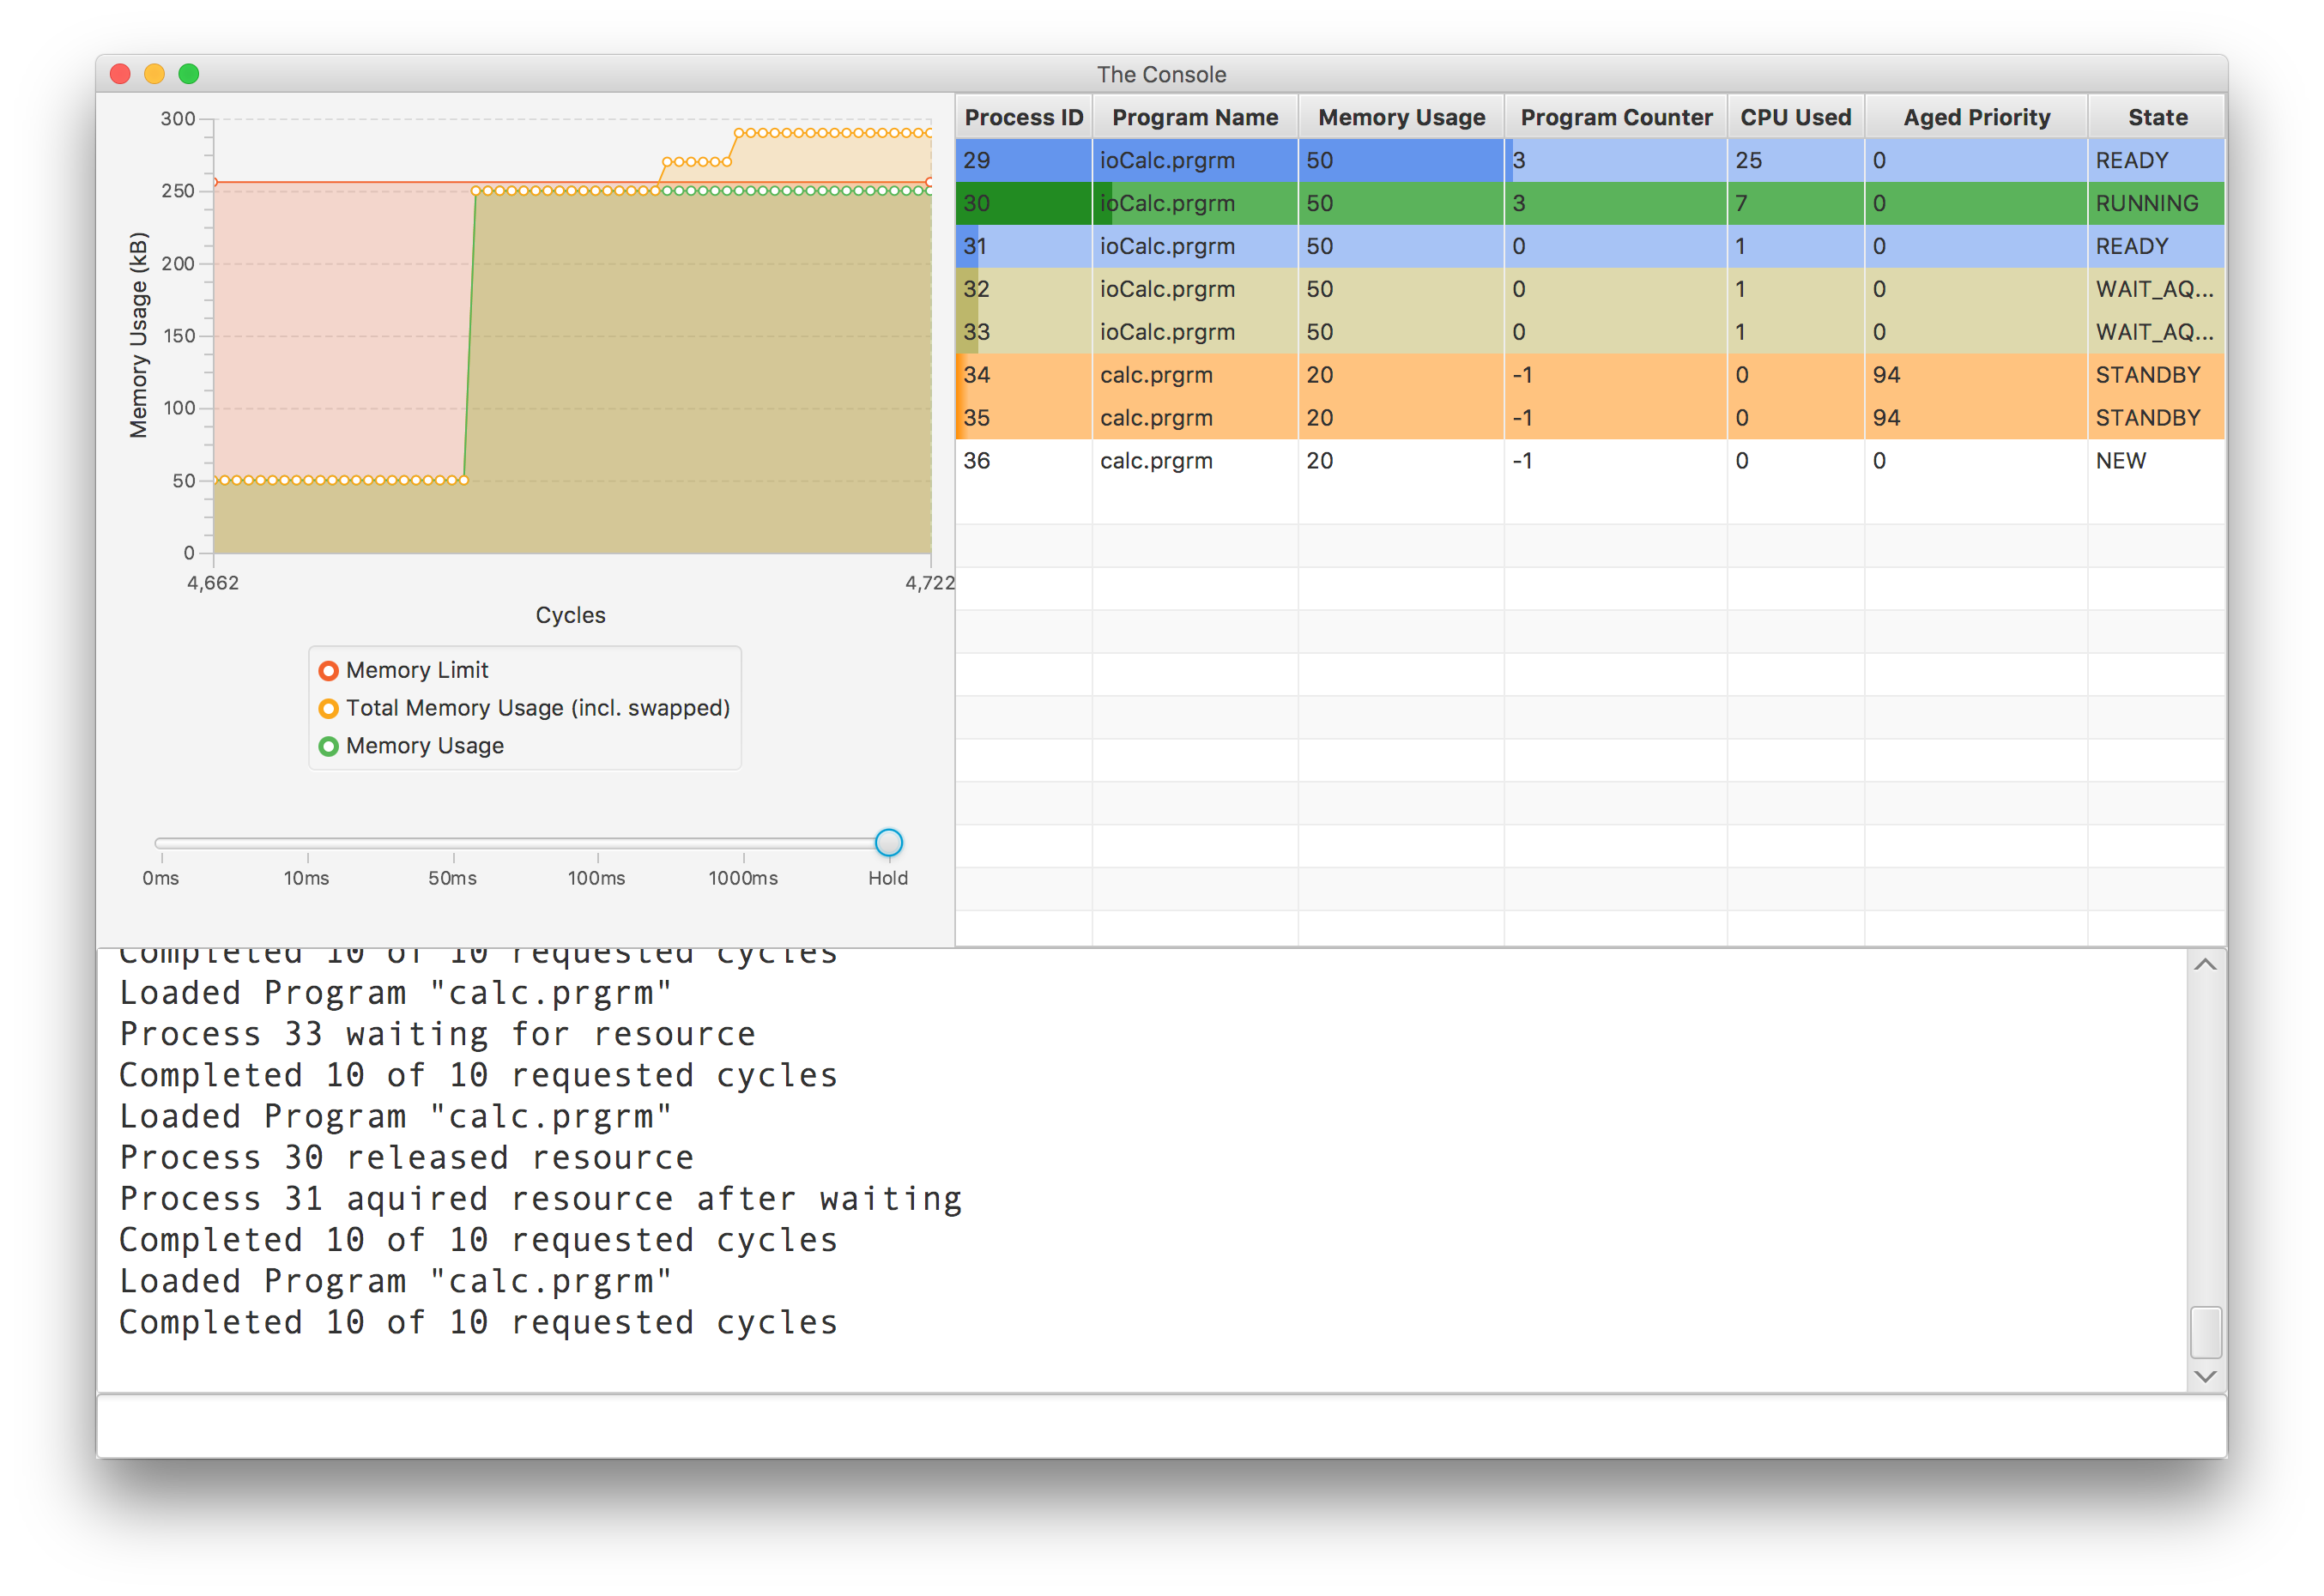
\includegraphics[width=\textwidth]{Demo.png} 

\end{document}
